\documentclass[10pt,a4paper]{article}
%% Language and font encodings
\usepackage[british]{babel}
\usepackage[utf8]{inputenc}
\usepackage[T1]{fontenc}
%% Sets page size and margins
\usepackage[a4paper,top=2cm,bottom=2cm,left=2.5cm,right=2.5cm,marginparwidth=1.5cm]{geometry}
%% Useful packages
\usepackage{amsmath}
\usepackage{graphicx}
\usepackage[colorinlistoftodos]{todonotes}
\usepackage[colorlinks=true, allcolors=blue,]{hyperref}
\usepackage{authblk}
\usepackage[backend=biber,style=numeric-comp]{biblatex}
\usepackage{listings}
\usepackage{xcolor}
\usepackage{amsmath} \allowdisplaybreaks% lets align equations break over pages.
\usepackage{amssymb}
\usepackage{caption}

\definecolor{codegreen}{rgb}{0,0.6,0}
\definecolor{codegray}{rgb}{0.5,0.5,0.5}
\definecolor{codepurple}{rgb}{0.58,0,0.82}
\definecolor{backcolour}{rgb}{0.95,0.95,0.92}


% \addbibresource{references.bib}

\lstdefinestyle{mystyle}{
  backgroundcolor=\color{backcolour}, 
    commentstyle=\color{codegreen},
    keywordstyle=\color{magenta},
    numberstyle=\tiny\color{codegray},
    stringstyle=\color{codepurple},
    basicstyle=\ttfamily\footnotesize,
    breakatwhitespace=false,         
    breaklines=true,                 
    captionpos=b,                    
    keepspaces=true,                 
    numbers=left,                    
    numbersep=5pt,                  
    showspaces=false,                
    showstringspaces=false,
    showtabs=false,                  
    tabsize=2
}
\lstset{style=mystyle}

\graphicspath{{./img/}}

%% Title
\title{
  {\Huge Simulation and Performance Evaluation}\\
  \huge Homework 3 \\
}

\author{Blascovich Alessio and Di Noia Matteo}

\begin{document}

\maketitle

\section*{Exercise 1}

\subsection*{Sub-exercises 1, 2 and 3}

\begin{center}
  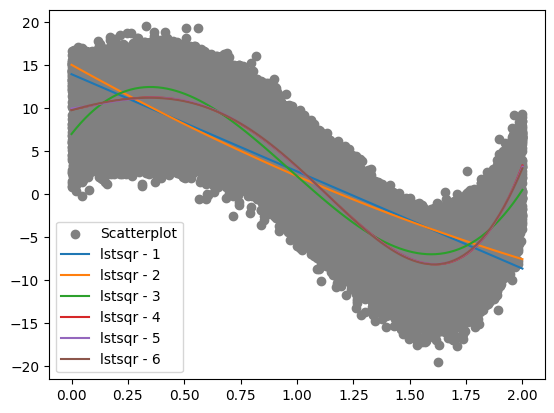
\includegraphics[width=0.5\textwidth]{point1.png}
  \captionof{figure}{Measurements and ``Least square'' trends for various ranks}
\end{center}

After drawing the the dataset scatter plot, it is clear that there is a trend in it. The trend is a sinusoidal-like curve with a local maximum after 0.3 seconds and a local minimum after 1.60 seconds. 

We used least square method to identify the trend. To be specific we used the polynomial fit with exponents between 1 and 6. We used:
\begin{itemize}
\item A \emph{Vandermonde}'s matrix called \emph{A} for the timestamps;
\item An array \emph{y} for the measurements taken.
\end{itemize}
The trend was represented by the array \(\hat{b} = (A^\prime A)^{-1} A^\prime y\). In our code the upper bound exponent for \emph{A} has been called \emph{rank}. For the sake of simplicity we handled all the matrix operations using the library \texttt{numpy}.

We iteratively increase the rank of the least squared function until, graphically, the curve was well fitted. Ranks before 4 gave us a poor fitting but from 4 we started seeing a well fitted curve so we decided to go once step further and use rank 5, even though 4 is probably enough.

%Ranks after 4 were practically indistinguishable from one another.

%Using the trend function with rank 5, even thou 4 is probably enough
The dataset has been de-trended by subtracting, the value of a polynomial function fitted over the \texttt{trend} array. Specifically, for each time point \emph{i}, the trend value at a given time was computed by evaluating the polynomial (whose coefficients are stored in the trend array) at the corresponding time \texttt{times[i]}. The de-trended measurement is then given by:

\begin{equation*}
  \texttt{measurements[i]} - \sum_{j = \texttt{len(trend)}}^{0}{\texttt{trend[j]} \cdot (\texttt{times[i]}^j)}
\end{equation*}

\begin{lstlisting}[language=python]
for i in range(len(measurements)):
    measurements[i] = measurements[i] - np.polyval(trend, times[i])
    # np.polyval evaluates a polynomial at specific values.
\end{lstlisting}

By drawing scatter plot of new data we showed that the trend was removed.% With the de-trended data the normalised histogram shows a distribution that can be fitted better.

\begin{minipage}[c]{0.5\textwidth}
    \centering
    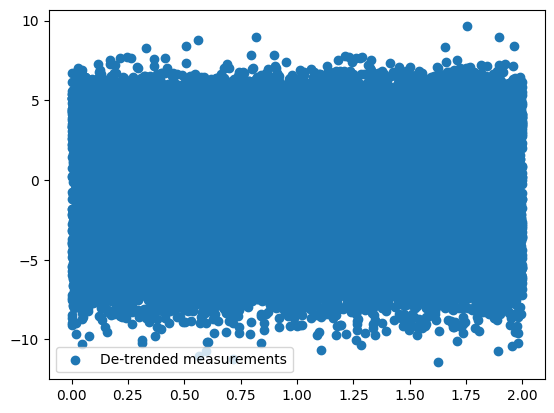
\includegraphics[width=\textwidth]{point2.png}
    \captionof{figure}{De-trended scatter plot}
\end{minipage}%
\begin{minipage}[c]{0.5\textwidth}
  \centering
  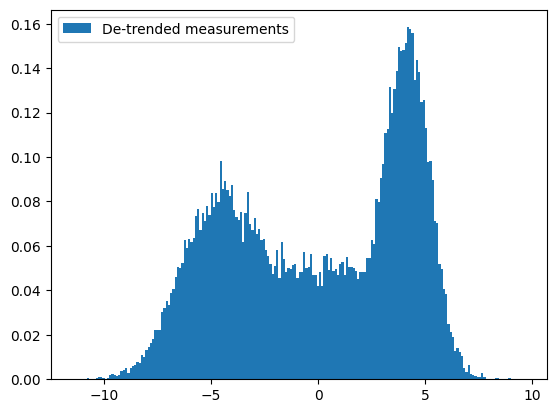
\includegraphics[width=\textwidth]{point3.png}
  \captionof{figure}{De-trended and normalised histogram}
\end{minipage}

\subsection*{Sub-exercise 4}

We started with three normal distributions:
\begin{itemize}
\item \(\mu = [-5, 0, 5]\);
\item \(\sigma = [1, 1, 1]\);
\item \(\text{probability} = [1/3, 1/3, 1/3]\).
\end{itemize}
%This were our starting assumptions about the distributions parameters. Note that, we could have picked better starting parameters, by using the histogram to get a better approximation of the means and variances. We avoided doing so because having looked to the real values we did not want to be influenced by them.

These were our initial assumptions about the Gaussians parameters. We could have done better by picking values closer to the values written on the homework text or by looking at the histogram.

We implemented the ``Expectation-Maximization'' following the procedures explained during the course. The algorithm proceeds iteratively through a series of iterations. During each iteration the algorithm computes the probability of a measurement to come from a specific Gaussian and then improves its assumptions about the parameters described above. In our implementation the probability of a point to be part of a Gaussian is updated as well. The resulting distribution fits quite well the dataset as shown in figure:

\begin{center}
  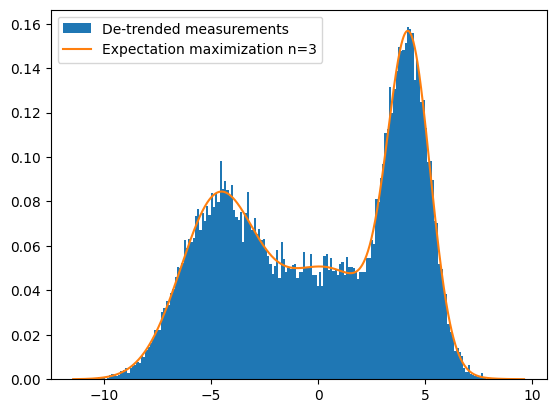
\includegraphics[width=0.5\textwidth]{point4.png}
  \captionof{figure}{Distribution produced by the E-M method}
\end{center}

The table below shows the results obtain by our algorithm compared against the given parameters. The estimators generated by our algorithm are: \(\overline{\text{X}}\) and \(\text{S}^2\), while the parameters given in the assignment text are: \(\mu\) and \(\sigma^2\). The comparison between our estimators and given parameters highlights that the mean estimators are slightly shifted to the right while the variance estimators are fairly precise. 

\begin{center}
  \begin{tabular}{c|c c c c c}
    & \(\overline{\text{X}}\) & \(\mu\) & \(\text{S}^2\) & \(\sigma^2\) & probability\\
    \hline
    Gaussian \# 1 & -4.72 & -5 & 3.07 & 3 & 0.345\\
    \hline
    Gaussian \# 2 & 0.410 & 0 & 5.96 & 6 & 0.302\\
    \hline
    Gaussian \# 2 & 4.26 & 4 & 0.980 & 1 & 0.353\\
    \hline
  \end{tabular}
\end{center}

\subsection*{Sub-exercise 5}

It is possible to automatically pick the best number of Gaussians to approximate the original distribution. The algorithm estimates the parameters for, an increasing, number \emph{n} of Gaussians using the ``Expectation-Maximization'' algorithm. For each iteration over \emph{n} we produced the T-value for the ``Chi-squared'' test, this value either stabilises as the mixture of Gaussians fits the dataset or increases again.% the T-value for the chi square test. This T-value grows smaller as the dataset fists better the sum of k-Gaussians.

We then defined the value \(\Delta\) which is the minimum improvement needed to continue the search for a better Gaussian. For each sum of Gaussians, after the first, we computed the improvement as: \[\frac{T - T^\prime}{T^\prime}\] where \(T^{\prime}\) is the T-value for the sum of \emph{n} Gaussians, while \(T\) is the T-value for the sum of \(k-1\) Gaussians. The algorithm continues its iteration over \emph{n} if \[\frac{T - T^\prime}{T^\prime} < \Delta\]% Once this condition is violated we check if \[P\{\chi^{2}_{k-1} \geq T^\prime\} < 0.05\] and if it is not the case, then the T-value stabilised around the value \emph{T} using \(k-1\) Gaussians.
Once this condition was violated we checked on ``Chi-squared'' tables for the value of \(P\{\chi^{2}_{k-1} \geq T^\prime\}\), if that value was \(\geq 0.05\) the we could not reject (neither accept) the hypothesis about the number \emph{n}. This part of the procedure can be automated as well using the function \texttt{chisquare} from the \texttt{numpy} library.

With \(\Delta = 0.01 = 1\%\), we got that a possible \emph{n} is 3, this can be easily seen in the following picture:

\begin{center}
  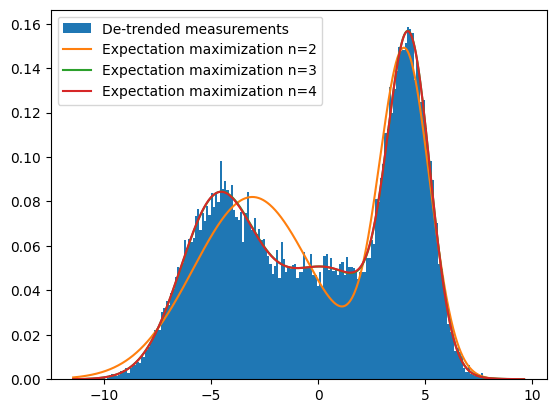
\includegraphics[width=0.5\textwidth]{point5.png}
  \captionof{figure}{Graphical representation of ``Chi-squared'' test}
\end{center}

% Because we computed the T-values we can then did the ``Chi-square'' test, for continuos functions, to verify if an hypothesis can be rejected. Doing so we can show that \(k = 2\) must be rejected while we cannot reject (neither accept) \(k = 3, 4\).
Using this procedure we shown that the hypothesis with \(n = 2\) must be rejected, while we could not reject (neither accept) the hypotheses \(n = 3, 4\).
\end{document}
